\setcounter{section}{0}
\part*{V. HƯỚNG DẪN VÀ LỜI GIẢI}
\addcontentsline{toc}{part}{V. HƯỚNG DẪN VÀ LỜI GIẢI}
\section{Đề 1}

\deda{
Giải bất phương trình $\sqrt{x^2+x}+\sqrt{x-2}\ge \sqrt{3(x^2-2x-2)}$.
}
\hda   
ĐK: $x\ge 1+\sqrt 3$.\\
Bình phương hai vế rút gọn ta được
$$ \sqrt{x(x+1)(x-2)}\ge x^2-4x-2\iff  \sqrt{(x^2-2x)(x+1)}\ge (x^2-2x)-2(x+1) $$
Phương trình có dạng $uv=u^2-2v^2\iff  (u+v)(2v-u)>0$ với $u+v>0$, nên ta suy ra được
$$ \sqrt{x^2-2x}\ge 2\sqrt{x+1}\iff  x^2-6x-4\ge 0\iff  x\in[3-\sqrt{13};3+\sqrt{13}]. $$
Kết hợp điều kiện ta được nghiệm của BPT là $[1+\sqrt 3;3+\sqrt{13}]$.

\deda{
\bd cho tam giác $OAB$ có các đỉnh $A,B$ thuộc đường thẳng $\Delta: 4x+3y-12=0$ và $K(6;6)$ là tâm đường tròn bàng tiếp góc $O$. Gọi $C$ là điểm nằm trên $\Delta$ sao cho $AC=AO$ và các điểm $C,B$ nằm khác phía nhau so với $A$. Biết $C$ có hoành độ bằng $\frac{24}5$, tìm tọa độ $A,B$.
}
\hda 
\begin{minipage}{0.42\textwidth}
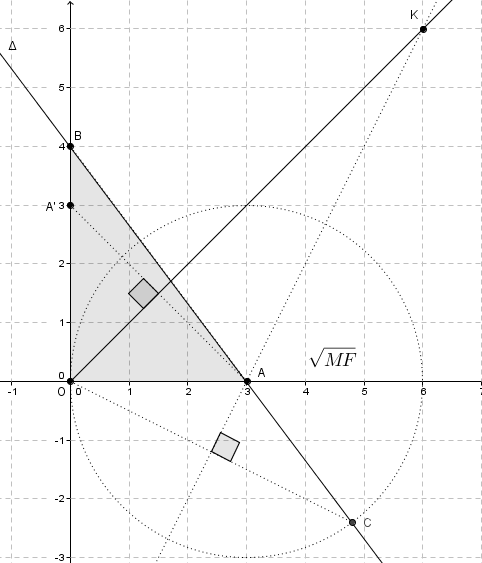
\includegraphics[scale=0.5]{de1.png}
\end{minipage}
\begin{minipage}{0.55\textwidth}
Ta có $x_C=\frac{24}5$, $C\in\Delta$ nên ta có tọa độ $C\left(-\frac{12}5;\frac{24}5\right)$.\\
Do $AO=AC$ nên $A$ nằm trên trung trực $d$ của $OC$. Với tọa độ $O,C$ đã biết ta tìm được $d$: $2x-y-6=0$.\\
Khi đó, $A=\Delta\cap d$ nên $A(3;0)$.\\
Ta có $K$ là tâm đường tròn bàng tiếp góc $O$ của tam giác $OAB$ nên $OK$ là phân giác góc $\goc{AOB}$. $OK$: $x-y=0$.\\
Gọi $A'$ là điểm đối xứng của $A$ qua $OK$, ta tìm được $A'(0;3)$ và $A'\in OB$. Do đó đường thẳng $OB$ chính là $Oy$ và ta tìm được $B(0;4)$.\\
\textit{\underline{Nhận xét}:} Với lời giải này ta thấy bài toán có một vài giả thiết thừa, chẳng hạn giả thiết tâm đường tròn bàng tiếp, giả thiết $C,B$ nằm khác phía so với $A$.
\end{minipage}

\deda{
 Cho $x\in \mathbb{R}$. Tìm GTNN của
$$ P=\dfrac{\sqrt{3(2x^2+2x+1)}}{3}+\dfrac{1}{\sqrt{2x^2+(3-\sqrt 3)x+3}}+\dfrac{1}{\sqrt{2x^2+(3+\sqrt 3)x+3}}. $$
}
\hda 
\bd với mỗi $x\in\mathbb{R}$ xét $A(x,x+1)$, $B\left(\frac{\sqrt 3}2;-\frac 12\right)$ và $C\left(-\frac{\sqrt 3}2;-\frac 12\right)$.\\
Khi đó ta có $P=\frac{OA}a+\frac{OB}b+\frac{OC}c$, trong đó $BC=a$, $CA=b$ và $AB=c$.\\
Gọi $G$ là trọng tâm $\Delta ABC$, ta có
$$ P=\frac{OA.GA}{a.GA}+\frac{OB.GB}{b.GB}+\frac{OC.GC}{c.GC}=\frac 32\left(\frac{OA.GA}{a.m_a}+\frac{OB.GB}{b.m_b}+\frac{OC.GC}{c.m_c}\right), $$
trong đó $m_a$, $m_b$, $m_c$ lần lượt là độ dài đường trung tuyến xuất phát từ $A,B,C$ của $\Delta ABC$.\\
Theo BĐT $AM-GM$, ta có
$$ a.m_a=\frac 1{2\sqrt 3}\sqrt{3a^2(2b^2+2c^2-a^2)}\le \frac 1{2\sqrt 3}\frac{3a^2+(2b^2+2c^2-a^2)}2=\frac{a^2+b^2+c^2}{2\sqrt 3}. $$
Bằng cách tương tự ta cũng có $b.m_b\le \frac{a^2+b^2+c^2}{2\sqrt 3}$ và $c.m_c\le \frac{a^2+b^2+c^2}{2\sqrt 3}$.\\
Suy ra $$P\ge \frac{3\sqrt 3}{a^2+b^2+c^2}(OA.GA+OB.GB+OC.GC).$$
Ta có $$OA.GA+OB.GB+OC.GC\ge \vt{OA}.\vt{GA}+\vt{OB}.\vt{GB}+\vt{OC}.\vt{GC}.$$
Mà
\begin{eqnarray*}
&&\vt{OA}.\vt{GA}+\vt{OB}.\vt{GB}+\vt{OC}.\vt{GC}\\
&=&\vt{OG}(\vt{GA}+\vt{GB}+\vt{GC})+GA^2+GB^2+GC^2\\
&=&\frac 49(m_a^2+m_b^2+m_c^2)=\frac{a^2+b^2+c^2}3
\end{eqnarray*}
Từ đó $P\ge 3$, đẳng thức xảy ra khi $x=0$. Vậy $P_{\min}=\sqrt 3$.
%Miễn bình luận.
\section{Đề 2}

\deda{
\bd cho hình vuông $ABCD$ có $M,N$ lần lượt là trung điểm của $BC$, $CD$. Tìm tọa độ $B, M$ biết $N(0;-2)$, đường thẳng $AM$ có phương trình $x+2y-2=0$ và cạnh hình vuông bằng $4$. 
}
\hda 
\begin{minipage}{0.5\textwidth}
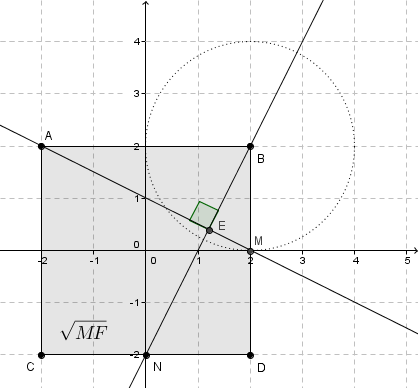
\includegraphics[scale=0.7]{de2-h1.png}
\end{minipage}
\begin{minipage}{0.5\textwidth}
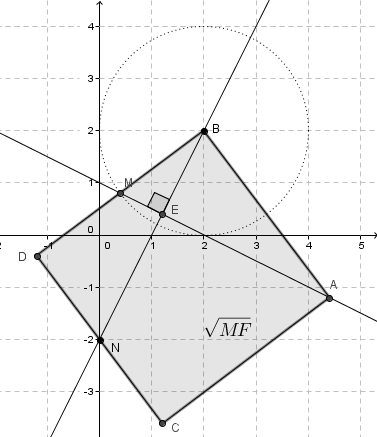
\includegraphics[scale=0.7]{de2-h2.png}
\end{minipage}
Chìa khóa của bài toán chính là tính chất $AM\bot BN$ (Tính chất này thường xuất hiện trong các đề thi đặc biệt thường xuất hiện với tư cách đáy của một hình chóp).\\
Trước hết $\Delta ABM\backsim \Delta BEM$ $(g.g)$ với $E=AM\cap BN$. Nên $AM\bot BN$.\\
Từ đó tìm được $BN$: $2x-y-2=0$ và $E\left(\frac 65;\frac 25\right)$.\\
Mặt khác ta cũng tính được $BE=\frac{4\sqrt 5}5$, $EN=\frac{6\sqrt 5}5$. Nên $\vt{EB}=-\frac 23\vt{EN}$, suy ra $B(2;2)$.\\
Lại có $BM=2$ nên $M$ thuộc đường tròn $(C)$ tâm $B$ bán kính $2$.
$(C)$: $(x-2)^2+(y-2)^2=4$.\\
$M=AM\cap (C)$ nên ta tìm được 2 điểm $M$ thỏa mãn: $M_1(2;0)$, $M_2\left(\frac 25;\frac 45\right)$.
\deda{
Giải hệ phương trình $\hpt{27x^3+3x+(9y-7)\sqrt{6-9y}=0\\ \frac 13x^2+y^2+\sqrt{2-3x}-\frac{109}{81}=0}$.
}
\hda 
Quan sát phương trình (1) của hệ ta thấy có thể độc lập thành hai phần, chỉ chứa $x$ và chỉ chứa $y$. Phần chứa $x$ có bậc $3$, phần chứa $y$ có dạng $u\sqrt{u}=(\sqrt{u})^3$ nên ta sẽ nghĩ đến việc dùng phương pháp hàm, với hàm đặc trưng là một hàm bậc 3.
 $$ (1)\iff  (3x)^3+3x=(6-9y)\sqrt{6-9y}+6-9y.\quad (\ast) $$
Dễ thấy hàm $f(t)=t^3+t$ đồng biến trên $\mathbb{R}$ nên
$$ (\ast)\iff  f(3x)=f(\sqrt{6-9y})\iff  3x=\sqrt{6-9y}\iff  \hpt{x\ge 0\\ y=\frac 23-x^2}. $$
Thế vào phương trình $(2)$ ta được $\frac 13 x^2+(\frac 23-x^2)^2+\sqrt{2-3x}-\frac{109}{81}=0$.\\
Vế trái của phương trình trên là hàm đồng biến trên $(0;\frac 23)$, lại thử thấy $x=\frac 13$ là một nghiệm nên hệ có nghiệm duy nhất $(\frac 13;\frac 59)$.

\deda{
 Tìm GTLN và GTNN của biểu thức $P=5^{2x}+5^y$, biết $x\ge 0$, $y\ge 0, x+y=1$.
}
\hda 
Ta có $x+y=1\iff  y=1-x$, nên $P=5^{2x}+\dfrac{5}{5^x}$.\\
Đặt $t=5^x$ thì $t\in [1;5]$. Xét $f(t)=t^2+\frac 5t$ với $t\in[1;5]$.\\
Ta tìm được $P_{\min}=f\left(\sqrt[3]{\frac 52}\right)=3\sqrt[3]{\frac{25}4}$, $P_{\max}=f(5)=26$.
\section{Đề 3}

\deda{
\bd hãy tính diện tích tam giác $ABC$ biết $H(5;5)$, $I(5;4)$ lần lượt là trực tâm và tâm đường tròn ngoại tiếp tam giác $ABC$ và cạnh $BC$ nằm trên đường thẳng $x+y-8=0$.
}
\hda 
\begin{minipage}{0.43\textwidth}
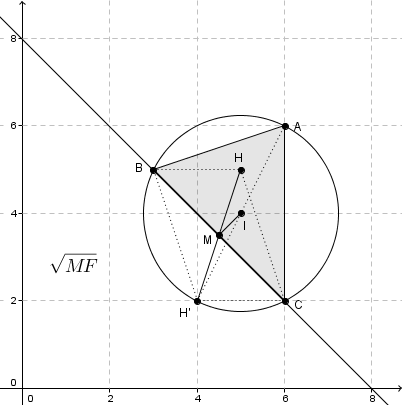
\includegraphics[scale=0.7]{de3.png}
\end{minipage}
\begin{minipage}{0.56\textwidth}
Đây là một dạng hình rất quen thuộc đối với các bạn lớp 9. Nói như thế để thấy rằng các bạn có kiễn thức hình phẳng lớp 9 tốt thì sẽ có lợi thế lớn trong chủ đề này.\\
Gọi $M$ là hình chiếu của $I$ lên $BC$, thì $M\left(\frac 92;\frac 72\right)$ và $M$ là trung điểm $BC$.\\
Gọi $H'$ là điểm đối xứng của $H$ qua $M$, thì $H'(2;4)$ và tứ giác $HBH'C$ là hình bình hành.\\
Do đó $H'C\parallel BH$, mà $BH\bot AC$ nên $\goc{ACH'}=90^o$, tương tự cũng có $\goc{ABH'}=90^o$. Suy ra tứ giác $ABH'C$ nội tiếp đường tròn đường kính $AH'$.
\end{minipage}\\
Từ đó $I$ là trung điểm của $AH'$, suy ra $A(6;6)$.\\
Lại có $BC=2MC=2\sqrt{R^2-MI^2}=3\sqrt 2$. Và $S_{\Delta ABC}=\frac 12d(A, BC).BC=6$.\\
\textit{\underline{Nhận xét}:} Ta có thể lấy điểm phụ $H'$ khác là giao của $AH$ với đường tròn ngoại tiếp tam giác.
\deda{
 Giải phương trình $(x-\ln x)\sqrt{2x^2+2}=x+1$.
}
\hda 
Đk: $x>0$. phương trình tương đương với $x-\ln x=\dfrac{x+1}{\sqrt{2x^2+2}}$.\quad $(\ast)$\\
Bằng cách xét hàm ta sẽ chỉ ra được $(\ast)$ có $VT\le 1$ và $VP\ge 1$, đẳng thức đều xảy ra khi $x=1$.\\
Vậy phương trình có nghiệm duy nhất $x=1$.

\deda{
Cho $0<x<y<z$. Tìm GTNN
$$ P=\dfrac{x^3z}{y^2(xz+y^2)}+\dfrac{y^4}{z^2(xz+y^2)}+\dfrac{z^3+15x^3}{x^2z}. $$
}
\hda 
Đặt $a=\frac xy$, $b=\frac yz$, $c=\frac zx$, suy ra $abc=1$, $c>1$ và
$$ P=\frac{\left(\frac xy\right)^3}{\frac xy+\frac yz}+\frac{\left(\frac yz\right)}{\frac xy+\frac yz}+\left(\frac zx\right)^2+\frac{15}{\frac zx}=\frac{a^3}{a+b}+\frac{b^3}{a+b}+c^2+\frac{15}c. $$
Ta có $a^3+b^3\ge ab(a+b)\implies  \frac{a^3}{a+b}+\frac{b^3}{a+b}\ge ab=\frac 1c$. Suy ra $P\ge \frac 1c+c^2+\frac{15}c=c^2+\frac{16}c$.\\
Xét $f(c)=c^2+\frac{16}c$ với $c\in (1;+\infty)$ ta được $f(c)\ge f(2)=12$.\\
Vậy $P_{\min}=12$ khi $z=\sqrt 2y=2x$.
\section{Đề 4}

\deda{
Giải hệ phương trình $\hpt{\sqrt{2x-y-1}+\sqrt{3y+1}=\sqrt x+\sqrt{x+2y}\\ x^3-3x+2=2y^3-y^2}.$
}
\hda 
Đk: $\hpt{2x\ge y+1\\ y\ge -\frac 13\\x\ge 0\\  x+2y\ge 0}\iff  \hpt{y\ge -\frac 13\\ x\ge \frac 13\\x+2y\ge 0}$.\\
Ở phương trình (1), quan sát các biểu thức dưới căn (hoặc sử dụng Casio), ta sẽ tìm được mối liên hệ giữa các biến định hướng cho các biến đổi sau
$$ (1)\iff  (\sqrt{2x-y-1}-\sqrt x)-(\sqrt{x-2y}-\sqrt{3y-1})=0$$
$$\iff  \dfrac{x-y-1}{\sqrt{2x-y-1}+\sqrt x}-\dfrac{x-y-1}{\sqrt{x-2y}+\sqrt{3y-1}}=0$$
$$\iff  \hoac{x-y-1=0\quad (3)\\ \sqrt{2x-y-1}+\sqrt x=\sqrt{x-2y}-\sqrt{3y-1}\quad (4)}. $$
$(3)\iff  y=x-1$ thế vào $(2)$ ta được phương trình bậc 3 ẩn $x$ có hai nghiệm $x=1$, $x=5$. Suy ra nghiệm hệ $(1;0)$ và $(5;4)$.\\
Với phương trình $(4)$, làm tương tự với $(1)$ ta sẽ có biến đổi
$$ (4)\iff  (\sqrt{2x-y-1}-\sqrt{x+2y})+(\sqrt x-\sqrt{3y-1})=0$$
$$\iff  \hoac{x-3y-1=0\\ \dfrac{1}{\sqrt{2x-y-1}+\sqrt{x+2y}}+\dfrac{1}{\sqrt x+\sqrt{3y-1}}=0\quad \textit{(Vô nghiệm)}} $$
Với $x-3y-1=0$ thế vào $(2)$ ta cũng sẽ tìm được $x=1$. Vậy hệ có hai nghiệm  $(1;0)$; $(5;4)$.

\deda{
\bd cho hình vuông $ABCD$ có tâm $I\left(\frac 72;\frac 32\right)$. Điểm $M(6;6)\in AB$ và $N(8;-2)\in BC$. Tìm tọa độ các đỉnh của hình vuông.
}
\hda 
\begin{minipage}{0.43\textwidth}
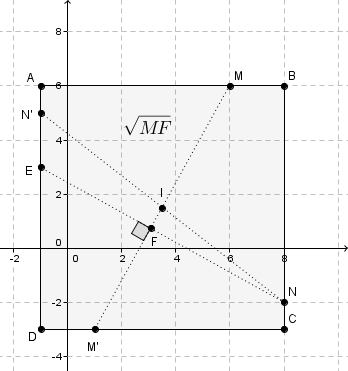
\includegraphics[scale=0.7]{de4.png}
\end{minipage}
\begin{minipage}{0.56\textwidth}
Ta tìm được tọa độ $M'(1;-3)$ đối xứng với $M$ qua $I$, $N'(-1;5)$ đối xứng với $N$ qua $I$.\\
Gọi $F$ là hình chiếu của $N$ lên $MM'$, do đã biết tọa độ $N$, viết được phương trình $MM'$ nên ta tìm được tọa độ $F\left(\frac{163}{53};\frac{39}{53}\right)$.\\
Mặt khác, ta lại chứng minh được $NE=MM'$ ($\Delta MM'P=\Delta NEQ$, với $P$ là hình chiếu của $M$ lên $CD$, $Q$ là hình chiếu của $N$ lên $AD$.).\\
Từ đó ta có $\vt{NF}=\frac{NF}{MM'}\vt{NE}$, do độ dài $NF$, $MM'$ tính được, tọa độ $N,F$ đã biết nên ta sẽ suy ra tọa độ $E(-1;3)$.\\
\end{minipage}\\
Khi đó ta viết được phương trình $AD$ (qua $E,N'$); phương trình $AB$, $CD$ ( lần lượt qua $M$, $M'$ vuông góc với $AD$) và tìm được tọa độ $A(-1;6)$, $D(-1;-3)$. Do $I$ là trung điểm $AC$, $BD$ nên cũng tìm được $C(8;-3)$, $B(8;6)$.
\deda{
Cho $x,y,z\in (0;1)$ thỏa mãn $(x^3+y^3)(x+y)=xy(1-x)(1-y)$. Tìm GTLN
$$ P=\dfrac{1}{\sqrt{1+x^2}}+\dfrac{1}{\sqrt{1+y^2}}+3xy-(x^2+y^2). $$
}
\hda 
Ta có $$ (x^3+y^3)(x+y)=xy(1-x)(1-y)\iff  \left(\frac{x^2}y+\frac{y^2}x\right)(x+y)=(1-x)(1-y). $$
Mà $\left(\frac{x^2}y+\frac{y^2}x\right)(x+y)\ge 4xy$ và $(1-x)(1-y)=1-(x+y)+xy\le 1-2\sqrt{xy}+xy$.\\
Suy ra $$1-2\sqrt{xy}+xy\ge 4xy\iff  0<xy\le\frac 19.$$
Mặt khác $\frac{1}{1+x^2}+\frac{1}{1+y^2}\le \frac{2}{1+xy}$ với $x,y\in (0;1)$. Suy ra
$$ \frac{1}{\sqrt{1+x^2}}+\frac{1}{\sqrt{1+y^2}}\le \sqrt{2\left(\frac{1}{1+x^2}+\frac{1}{1+y^2}\right)}\le\sqrt{2\left(\frac{2}{1+xy}\right)}=\frac{2}{\sqrt{1+xy}}. $$
Lại có $3xy-(x^2+y^2)=xy-(x-y)^2\le xy$. Suy ra $ P\le \frac{2}{\sqrt{1+xy}}+xy$.\\
Xét $f(t)=\frac{2}{\sqrt{1+t}}+t$ với $t\in\left(0;\frac 19\right]$. Ta tìm được $P_{\max}=f(\frac 19)=\frac{6\sqrt{10}}{10}+\frac 19$.
\section{Đề 5}

\deda{
\bd cho tam giác $ABC$ có trực tâm $H(-1;3)$, tâm đường tròn ngoại tiếp $I(-3;3)$, chân đường cao kẻ từ đỉnh $A$ là điểm $K(-1;1)$. Tìm tọa độ $A,B,C$.
}
\hda 
Ta có thể viết được phương trình $BC$ (qua $K$ vuông góc với $KH$) là $y-1=0$. Đến đây bạn đọc có thể tham khảo hướng dẫn giải ở \textbf{Đề 3} để tìm ra lời giải.\\
Ta tìm được $\{A(-1;7), B(1;1), (-7;1)\}$ hoặc $\{A(-1;7), B(-7;1), (1;1)\}$.

\deda{
Giải hệ phương trình $\hpt{x^2(x-3)-y\sqrt{y+3}=-2\\ 3\sqrt{x-2}=\sqrt{y(y+8)}}$.
}
\hda 
Đk: $x\ge 2$; $y\ge 0$\\
Quan sát $(1)$ ta cũng sẽ định hướng được sẽ sử dụng phương pháp hàm số, với hàm đặc trưng sẽ là một hàm bậc 3.
$$ (1)\iff  (x-1)^3-3(x-1)=(y+3)\sqrt{y+3}-3\sqrt{y+3}.\quad (\ast) $$
Dễ thấy hàm $f(t)=t^3-3t$ đồng biến trên $[1;+\infty)$ nên
$$ (\ast)\iff  f(x-1)=f(\sqrt{y+3})\iff  x-1=\sqrt{y+3} $$
Khi đó,
$$ (2)\iff  9(x-2)=y^2+8y\iff  9(\sqrt{y+3}-1)=y^2+8y\quad (\ast\ast) $$
Nhẩm (hoặc sử dụng Casio) tìm được nghiệm $y=1$ nên bằng phương pháp nhân liên hợp ta sẽ biến đổi được như sau
$$ (\ast\ast)\iff  (y-1)\left(\dfrac{9}{\sqrt x{y+3}+2}-y-9\right)=0\iff  y=1. $$
(Vì với $y\ge 0$ thì $\dfrac{9}{\sqrt x{y+3}+2}-y-9<0$). Vậy hệ có nghiệm $(3;1)$.

\deda{
Cho $x,y,z\in \mathbb{R}$ thỏa mãn $x^2+y^2+z^2=9$, $xyz\le 0$. CMR $2(x+y+z)-xyz\le 10$.
}
\hda 
Không giảm tính tổng quát, giả sử $x\le y\le z$, do $xyz\le 0$ nên $x\le 0$. Lại có $x^2+y^2+z^2=9$ nên $x^2\le 9$, suy ra $x\in [-3;0]$.\\
Mặt khác $yz\le \left(\frac{y+z}2\right)^2\le \frac{y^2+z^2}2$. Do đó 
\begin{eqnarray*}
&&2(x+y+z)-xyz\\ 
&=& 2x+2(y+z)-xyz\\
&\le & 2x+2\sqrt{2(y^2+z^2)}-x\cdot \frac{y^2+z^2}2\\
&=&\frac 12x^3-\frac 52 x+2\sqrt{2(9-x^2)}=f(x).
\end{eqnarray*}
Xét $f(x)$ trên $[-1;0]$ ta sẽ chỉ ra điều phải chứng mình. Đẳng thức xảy ra khi $x=-1, y=z=2$.
\section{Đề 6}

\deda{
\bd cho tam giác $ABC$ có tâm đường tròn ngoại tiếp là $I(-2;1)$ và thỏa mãn điều kiện $\goc{AIB}=90^o$, chân đường cao kẻ từ $A$ đến $BC$ là $D(-1;-1)$, đường thẳng $AC$ đi qua $M(-1;4)$. Tìm tọa độ $A,B$ biết $A$ có hoành độ dương.
}
\hda 
\begin{minipage}{0.43\textwidth}
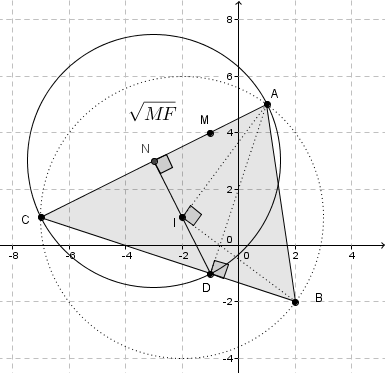
\includegraphics[scale=0.7]{de6.png}
\end{minipage}
\begin{minipage}{0.56\textwidth}
Chìa khóa của bài toán là có lẽ là phát hiện ra mối liên hệ giữa 3 giả thiết bài toán đã cho: $DI\bot AC$ ($M\in AC$). Việc định hướng được tính chất này cũng khá tự nhiên, nhưng cần kiến thức hình lớp 9 vững, đây cũng là xu hướng ra đề thường gặp.\\
Ta có $\goc{AIB}=90^o$ nên $\goc{ACB}=45^o$ (Góc nội tiếp bằng $\frac 12$ góc ở tâm cùng chắn cung). Do đó $\Delta ACD$ vuông cân tại $D$, suy ra $DA=DC$, mà $IA=IC$ nên $DI$ là đường trung trực của $AC$.\\
Từ đó, $ID\bot AC$ và $N$ là trung điểm $AC$ với $N$ là hình chiếu vuông góc của $I$ lên $AC$.
\end{minipage}\\
Ta tìm được $AC$: $x-2y+9=0$ (qua $M$ vuông góc với $DI$) và $N(-3;3)$. Ta cũng viết được phương trình đường tròn $(C)$: $(x+3)^2+(y-3)^2=20$ tâm $N$ bán kính $ND$. Suy ra $A(1;5)=(C)\cap AC$ (chú ý, hoành độ $A$ dương) và cũng sẽ tìm được $B(2;-2)$.
\deda{
Giải BPT $3(x^2-2)+\dfrac{4\sqrt 2}{\sqrt{x^2-x+1}}>\sqrt x(\sqrt{x-1}+3\sqrt{x^2-1})$.
}
\hda 
Đk: $x\ge 1$, ta biến đổi phương trình trở thành
$$ 3(\sqrt{x^2-1}-\sqrt{x})^2+(\sqrt{x^2-x}-1)^2+2\left(\dfrac{4\sqrt 2}{\sqrt{x^2-x+1}}+x^2-x-5\right)>0.\quad (\ast) $$
Xét hàm $f(t)=\dfrac{4\sqrt 2}{t}+t^2-6$ với $t=\sqrt{x^2-x+1}\ge 1$.\\ Ta có $f'(t)=2t-\dfrac{4\sqrt 2}{t^2}=\dfrac{2(t^3-2\sqrt 2)}{t^2}$,\quad $f'(t)=0\iff  t=\sqrt 2$.\\
Lập bảng biến thiên và ta sẽ chỉ ra được $f(t)\ge 0$ với mọi $t\ge 1$.\\
Đẳng thức xảy ra khi $t=\sqrt 2\iff  x=\dfrac{1+\sqrt 5}2$.\\
Từ đó ta có $(\ast)\iff  \hoac{\sqrt{x^2-1}-\sqrt x\neq 0\\ \sqrt{x^2-x}-1\neq 0\\ \dfrac{4\sqrt 2}{\sqrt{x^2-x+1}}+x^2-x-5\neq 0}\iff  x\neq \dfrac{1+\sqrt5}{2}$.\\
Vậy tập nghiệm của phương trình là $S=[1;+\infty)\setminus\left\{\dfrac{1+\sqrt 5}2\right\}$.
%Nhận xét: Bài tập như dở hơi -_-

\deda{
Xét các số thực dương $x,y,z$ thỏa mãn điều kiện $2(x+y)+7z=xyz$. Tim GTNN $S=2x+y+2z$.
}
\hda 
Ta có $2(x+y)=z(xy-7)$. Do $x,y,z$ là các số dương nên $xy-7>0$, suy ra $z=\frac{2(x+y)}{xy-7}$.\\
Suy ra $S=f(x,y)=2x+y+\frac{4(x+y)}{xy-7}$ với điều kiện $x>0$, $y>0$, $xy>7$.\\
Với mỗi $x$ cố định, xét đạo hàm của $f(x,y)$ theo ẩn $y$ ta được:
$$ f'_y(x,y)=1+\frac{4(xy-7)-4x(x+y)}{(xy-7)^2}=1-\frac{28+4x^2}{(xy-7)^2}. $$
Khi đó, $f'_y(x,y)=0\iff  x^2y^2-14xy+21-4x^2=0\iff  y_o=\frac 7x+2\sqrt{1+\frac 7{x^2}}$.\\
Suy ra $$f(x,y)\ge f(x,y_o)=2x+\frac{11}x+4\sqrt{1+\frac 7{x^2}}=g(x).$$
Xét $g(x)$ với $x\in (0;+\infty)$ ta sẽ tìm được $S\ge f(x;y_o)=g(x)\ge 15$.\\
Vậy $S_{\min}=15$ khi $x=3$, $y=5$, $z=2$.
\section{Đề 7}

\deda{
\bd cho hình bình hành $ABCD$ có $N$ là trung điểm $CD$ và $BN$ có phương trình $13x-10y+13=0$; điểm $M(-1;2)$ thuộc đoạn thẳng $AC$ sao cho $AC=4AM$. Gọi $H$ là điểm đối xứng của $N$ qua $C$. Tìm tọa độ $A,B,C,D$ biết $3AC=2AB$ và $H\in \Delta: 2x-3y=0$.
}
\hda 
\begin{minipage}{0.47\textwidth}
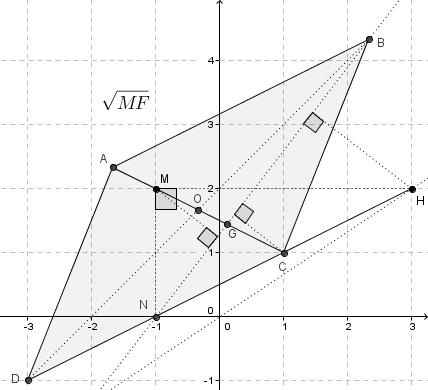
\includegraphics[scale=0.7]{de7.png}
\end{minipage}
\begin{minipage}{0.5\textwidth}
Gọi $G=BN\cap AC$ thì $G$ là trọng tâm tam giác $BCD$, suy ra $GC=\frac 13AC$. Mà $AC=4AM$ nên $MG=\frac 5{12}AC$, suy ra $CG=\frac 45MG$.
Từ đó $$d(C, BN)=\frac 45d(M,BN).$$
Lại có $HN=2CN$ nên $$d(H,BN)=2d(C,BN)=\frac 85d(M,BN).$$
Mà $d(M,BN)=\frac{20}{\sqrt{269}}$ và $H(3t,2t)$ (do $H\in\Delta$). Nên ta sẽ tìm được $t=1$, $t=-\frac{45}{19}$.
\end{minipage}\\
Để ý rằng $M, H$ nằm khác phía so với $BN$ nên ta chỉ ra được $H(3;2)$.\\
Mặt khác với giả thiết $3AC=2AB=2CD=2NH$ ta chỉ ra được $MC=\frac 12NH$ tức là tam giác $MNH$ vuông tại $M$ và tìm được $N(-1;0)$.\\
Từ đó ta sẽ tìm được $C(1;1)$, $D(-3;-1)$, $A\left(-\frac 53;\frac 73\right)$, $B\left(\frac 73;\frac{13}3\right)$.

\deda{
Giải hệ phương trình $\hpt{x^2+(y^2-y-1)\sqrt{x^2+2}-y^3+y+2=0\\ \sqrt[3]{y^2-3}-\sqrt{xy^2-2x-2}+x=0}.$
}
\hda 
Đk: $xy^2-2x-2\ge 0$.\\
Trong phương trình $(1)$, đặt $\sqrt{x^2+2}=t\ge 2$ ta được
$$ t^2+(y^2-y-1)t-y^3+y=0.\quad (\ast) $$
Do $\Delta_t=(y^2+y-1)^2$ (hoặc sử dụng Casio) nên
$$ (\ast)\iff \hoac{t=y\\ t=1-y^2\le 1\,\,\textit{(loại)}}\iff \hpt{y\ge 2\\ y^2=x^2+2}. $$
Thế vào $(2)$ ta được
$$ \sqrt[3]{x^2-1}-\sqrt{x^3-2}+x=0\quad\quad\text{(Đk: $x\ge\sqrt[3]{2}$).} $$
Bằng phương pháp nhân với lượng liên hợp ta sẽ chỉ ra được phương trình trên có đúng 1 nghiệm $x=3$.
\deda{
Cho $a\in[1;2]$. CMR $(2^a+3^a+4^a)(6^a+8^a+12^a)<24^{a+1}$.
}
\hda 
Bất đẳng thức tương đương với $$ (2^a+3^a+4^a)\left(\frac 1{2^a}+\frac 1{3^a}+\frac 1{4^a}\right)<24. $$
Do $a\in[1;2]$ nên $2\le 2^a\le 4$; $3\le 3^a\le 9$; $4\le 4^a\le 16$ $\implies $ $2\le 2^a<16$; $2<3^a<16$; $2<4^a\le 16$.\\
Lại có, $x\in[2;16]$ thì $(x-2)(x-16)\le 0\iff  x^2-18x+32\le 0\iff  x-18+\frac{32}x\le 0\iff  \frac{32}x\le 18-x$.\\
Từ đó suy ra
$$ 32\left(\frac 1{2^a}+\frac 1{3^a}+\frac 1{4^a}\right)<54-(2^a+3^a+4^a)\iff   \frac 1{2^a}+\frac 1{3^a}+\frac 1{4^a}<\frac{54-(2^a+3^a+4^a)}{32}.$$
Khi đó
\begin{eqnarray*}
(2^a+3^a+4^a)\left(\dfrac 1{2^a}+\dfrac 1{3^a}+\dfrac 1{4^a}\right)&<&\dfrac{(2^a+3^a+4^a)[54-(2^a+3^a+4^a)]}{32}\\ 
& \le & \dfrac{1}{32}\left[\dfrac{[2^a+3^a+4^a+54-(2^a+3^a+4^a)]}{2}\right]^2=\dfrac{729}{32}<24.
\end{eqnarray*}
\section{Đề 8}

\deda{
\bd cho hình bình hành $ABCD$ có $\goc{ABC}$ nhọn, $A(-2;-1)$. Gọi $H,K,E$ lần lượt là hình chiếu vuông góc của $A$ trên các đường thẳng $BC, BD, CD$. Đường tròn $(C):$ $x^2+y^2+x+4y+3=0$ ngoại tiếp tam giác $HKE$. Tìm tọa độ $B,C,D$ biết $H$ có hoành độ âm, $C$ có hoành độ dương và nằm trên đường thẳng $x-y-3=0$.
}
\hda 
\begin{minipage}{0.47\textwidth}
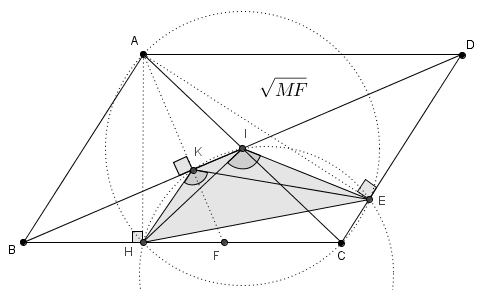
\includegraphics[scale=0.6]{de8.png}
\end{minipage}
\begin{minipage}{0.52\textwidth}
Gọi $I=AC\cap BD$, ta sẽ chứng minh $I\in (C)$ bằng cách chỉ ra $HKIE$ là tứ giác nội tiếp. Thật vậy, $AHCE$ nội tiếp đường tròn tâm $I$ nên $\goc{HIE}=2\goc{HAE}$ (góc ở tâm và góc nội tiếp cùng chắn 1 cung).\\
Lại có $ABHK, AKED$ là các tứ giác nội tiếp và $\goc{EAB}=\goc{HAD}=90^o$ nên 
\end{minipage}
$$\goc{HKE}=180^o-\goc{HKB}-\goc{EKD}=180^o-\goc{HAB}-\goc{EAD}=90^o-\goc{HAB}+90^o-\goc{EAD}=2\goc{HAE}.$$
Từ đó, $\goc{HKE}=\goc{HIE}$, tức là $HKIE$ nội tiếp.\\
Mặt khác, $I$ là trung điểm $AC$ và $C(c;c-3)\in d$ $(c>0)$ nên $I\left(\frac{c-2}2;\frac{c-4}2\right)$. Do $I\in (C)$ nên ta tìm được $c=2$ và $I(0;-1)$, $C(2;-1)$.\\
Gọi $(C')$ là đường tròn đường kính $AC$, $(C')$: $x^2+(y+1)^2=4$.\\
$E,H=(C)\cap (C')$ nên ta sẽ tìm được $\left(-\frac 85;-\frac{11}5\right)$, $E(0;-3)$ (Do $H$ có hoành độ âm). \\
Từ đó ta cũng tìm được $B(-4;-3)$, $C(2;-1)$, $D(4;1)$.
\deda{
Giải hệ phương trình $\hpt{3\sqrt{y^3(2x-y)}+\sqrt{x^2(5y^2-4x^2)}=4y^2\quad (1)\\ \sqrt{2-x}+\sqrt{y+1}+2=x+y^2\quad (2)}$.
}
\hda 
Đk: $x\le 2$; $y\ge -1$; $y^3(2x-y)\ge 0$; $5y^2-4x^2\ge 0$.\\
Nhận thấy $(1)$ đồng bậc $3$ nên đặt $y=tx$. Ta có $y^3(2x-y)\ge 0\implies  xy\ge 0\implies  t> 0$.\\
Ta sẽ được phương trình
$$ 3\sqrt{t^3(2-t)}+\sqrt{5t^2-4}=4t^2. $$
Bằng phương pháp nhân với lượng liên hợp với nhân tử chung là $(t-1)^2$ ta xác định được $(\ast)$ có đùng một nghiệm $t=1$, tức là $x=y$. (Bằng BĐT AM-GM ta cũng sẽ chỉ ra được $x=y$).\\
Thế vào $(2)$ ta được
$$ \sqrt{2-x}+\sqrt{x+1}+2=x+x^2. $$
Suy ra $x^2+x-2>0\implies  x>1$. Bằng phương pháp nhân liên hợp ta sẽ phân tích phương trình trở thành
$$ (x^2-x-1)\left(1+\dfrac{1}{x-1+\sqrt{2-x}}+\dfrac{1}{x+\sqrt{x+1}}\right)=0 $$
$$ \iff  x^2-x-1=0\implies  x=y=\dfrac{1+\sqrt{5}}2. $$
\deda{
Cho $a,b,c>0$ thỏa mãn $4(a^3+b^3)+c^3=2(a+b+c)(ac+bc-2)$. Tìm GTLN
$$ P=\dfrac{2a^2}{3a^2+b^2+2a(c+2)}+\dfrac{b+c}{a+b+c+2}-\dfrac{(a+b)^2+c^2}{16}. $$
}
\hda 
Ta có $x^3+y^3\ge \frac 14(x+y)^3$; $xy\le \left(\frac{x+y}2\right)^2$ với mọi $x,y>0$. Suy ra
$$ \frac 14(a+b+c)^3\le (a+b)^3+c^3\le 4(a^3+b^3)+c^3\le 2(a+b+c)\left(\frac{(a+b+c)^2}4-2\right) $$
Suy ra $a+b+c\ge 4$.\\
Khi đó áp dụng BĐT AM-GM ta có
$$ \frac{2a^2}{3a^2+b^2+2a(c+2)}=\frac{a}{a+c+2+\left(\frac{b^2}{2a}+\frac a2\right)}\le \frac{a}{a+c+2+2\sqrt{\frac{b^2}{2a}\cdot\frac a2}}=\frac a{a+b+c+2}, $$
và $(a+b)^2+c^2\ge \frac 12(a+b+c)^2$. Suy ra $$P\le \frac{a+b+c}{a+b+c+2}-\frac{(a+b+c)^2}{32}=\frac{t}{t+2}-\frac{t^2}{32}.$$
Với $t=a+b+c\ge 4$, ta có $f'(t)=\frac{2}{(t+2)^2}-\frac{t}{16}=\frac{32-t(t+2)^2}{16(t+2)^2}<0$, $\forall t\ge 4$.\\
Suy ra $f(t)$ nghịch biến trên $[4;+\infty)$. Do đó $P\le f(t)\le f(4)=\frac 16$.\\
Dấu bằng xảy ra khi $\hpt{a=b,a+b=c\\ a+b+c=4}\iff  a=b=1,c=2$. Vậy $P_{\max}=\frac 16$.
\section{Đề 9}

\deda{
Giải hệ phương trình $\hpt{\sqrt{x+2y+1}-2x=4(y-1)\quad (1)\\ x^2+4y^2+2xy=7\quad (2)}$.
}
\hda 
Đây là một hệ phương trình khá đơn giản.\\
Với $(1)$, đặt $\sqrt{x+2y+1}=t$, ta sẽ giải được $t=2$. Thế vào $(2)$ ta tìm được nghiệm của hệ là $(1;1)$ và $(1;\frac 12)$.

\deda{
\bd cho tam giác $ABC$ có phương trình đường thẳng $AB$: $2x+y-1=0$, phương trình $AC:$, $3x+4y+6=0$ và điểm $M(1;-3)$ nằm trên $BC$ thỏa mãn $3MB=2MC$. Tìm tọa độ trọng tâm $G$ của tam giác $ABC$.
}
\hda 
Một bài tập khá đơn giản minh họa cho phương pháp tham số hóa.\\
$A=AB\cap AC$ nên $A(2;-3)$. $B\in AB$ nên $B(b;1-2b)$, $C\in AC$ nên $C(-2-4c;3c)$.\\
 Một điểm lưu ý là $M$ chưa biết nằm trong hay nằm ngoài $B,C$ nên ta cần xét 2 trường hợp\\
\textbf{TH1}: $M$ nằm ngoài, tức là $3\vt{MB}=2\vt{MC}$ ta tìm được $b=\frac{11}5$, $c=-\frac 65$. Từ đó $G\left(\frac 73;-\frac{10}3\right)$.\\
\textbf{TH2}: $3\vt{MB}=-2\vt{MC}$ ta cũng xác định được $G\left(1;-\frac 83\right)$.

\deda{
Tìm tất cả các giá trị của $m$ để bất phương trình sau có nghiệm trên $[0;2]$
$$ \sqrt{(m+2)x+m}\ge |x-1|. $$
}
\hda 
Với $x\in [0;2]$ ta có $$\sqrt{(m+2)x+m}\ge |x-1|\iff  (m+2)x+m\ge (x-1)^2\iff  m\ge \frac{x^2-4x+1}{x+1}=f(x).$$
Xét $f(x)$ trên $[0;2]$ ta chỉ ra được $f(x)\in [2\sqrt 6-6;1]$.\\
Do đó để BPT có nghiệm trên $[0;2]$ thì $m\ge 2\sqrt 6-6$.
\section{Đề 10}

\deda{
\bd cho hình vuông $ABCD$ có $A(-1;2)$. Gọi $M, N$ lần lượt là trung điểm của $AD$ và $DC$; $K=BN\cap CM$. Viết phương trình đường tròn ngoại tiếp tam giác $BMK$, biết $BN$ có phương trình $2x+y-8=0$ và điểm $B$ có hoành độ lớn hơn $2$. 
}
\hda 
\begin{minipage}{0.3\textwidth}
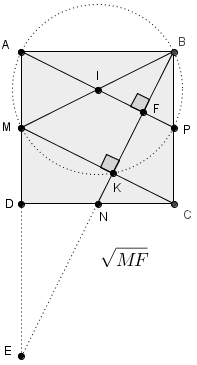
\includegraphics[scale=0.9]{de10.png}
\end{minipage}
\begin{minipage}{0.68\textwidth}
Một lần nữa, chúng ta lại bắt gặp tính chất hình học ở \textbf{Đề 2}, tuy nhiên cần phải tận dụng nó một cách khéo léo kết hợp với các giả thiết khác.\\
Tương tự như ở \textbf{Đề 2}, ta chứng minh được $CM\bot BN$ và $AP\bot BN$ với $P$ là trung điểm $BC$. Và do đó, $I=AP\cap BM$ là tâm của đường tròn ngoại tiếp $\Delta BKM$ có đường kính $BM$.\\
Mặt khác, gọi $F=AP\cap BN$ ta có $AF=d(A,BN)=\frac8{\sqrt 5}$.\\
Gọi $E=AD\cap BN$, dễ thấy $D$ là trung điểm $AE$. Lại có $$\frac 1{AF^2}=\frac 1{AB^2}+\frac{1}{AE^2}=\frac 5{4AB^2}.$$
Nên $AB=4$. Từ đó ta tính được $IA=\frac{AP}2=\sqrt 5$, suy ra $\vt{AI}=\frac 58\vt{AF}$. Ta lại tìm được $F\left(\frac{11}5;\frac{18}5\right)$ (Hình chiếu của $A$ lên $BN$) nên ta cũng tính được $I(1;3)$. Và phương trình cần tìm là $(x-1)^2+(y-3)^2=5$.
\end{minipage}

\textit{\underline{Nhận xét}:} Cách làm trong đáp án chính thức cần tìm tọa độ điểm $B$ từ giả thiết $AB=4$ và $B\in BN$ nên cần $x_B>2$ để loại nghiệm. Nhưng với cách làm này ta thấy giả thiết $x_B>2$ bị thừa.


\deda{
Giải hệ phương trình $\hpt{(1-y)\sqrt{x^2+2y^2}=x+2y+3xy\quad (1)\\ \sqrt{y+1}+\sqrt{x^2+2y^2}=2y-x\quad (2)}$.
}
\hda 
Đk: $y\ge -1$. Với phương trình $(1)$, đặt $\sqrt{x^2+2y^2}=t\ge 0$, coi là phương trình ẩn $t$, $x,y$ là tham số. Ta tính được $\Delta_t=(2x+3y+1)^2$ nên
$$(1)\iff  \hoac{\sqrt{x^2+2y^2}=-x-y-1\\ \sqrt{x^2+2y^2}=x+2y}$$
Thế vào $(2)$ ta được nghiệm $\left(\dfrac{-1-\sqrt 5}4;\dfrac{1+\sqrt 5}2\right)$.
% Nx: Bài toán mang tính chất đánh đố.
\deda{
Cho $x,y,z>0$ thỏa mãn $5(x^2+y^2+z^2)=9(xy+2yz+zx)$. Tìm GTLN
$$ P=\dfrac{x}{y^2+z^2}-\dfrac{1}{(x+y+z)^3}. $$
}
\hda 
Ta có $5x^2+5(y^2+z^2)=9x(y+z)+18yz\iff  5x^2-9x(y+z)=18yz-5(y^2+z^2)$.\\
Lại có $yz\le \frac 14(y+z)^2$; $y^2+z^2\ge \frac 12(y+z)^2$ nên $18yz-5(y^2+z^2)\le 2(y+z)^2$.\\
Do đó
\begin{eqnarray*}
&&5x^2-9x(y+z)\le 2(y+z)^2\\ 
&\iff  & [x-2(y+z)](5x+y+z)\le 0\\
&\iff  & x\le 2(y+z). 
\end{eqnarray*}
Và
$$ P=\frac{x}{y^2+z^2}-\frac{1}{(x+y+z)^3}\le \frac{2x}{(y+z)^2}-\frac 1{(x+y+z)^3}\le \frac 4{y+z}-\frac 1{27(y+z)^3}. $$
Đặt $y+z=t>0$ ta có $P\le 4t-\frac 1{27}t^3=f(t)$. Xét $f(t)$ ta suy ra được $P\le 16$.\\
Vậy $P_{\max}=16$ khi $x=\frac 13$; $y=z=\frac 1{12}$.
\section{Đề 11}

\deda{
\bd cho hình thang $ABCD$ có đáy lớn $CD=2AB$, điểm $C(-1;-1)$, trung điểm của $AD$ là $M(1;-2)$. Tìm tọa độ $B$, biết diện tích tam giác $BCD$ bằng $8$, $AB=4$ và $D$ có hoành độ nguyên dương.
}
\hda 
\begin{minipage}{0.4\textwidth}
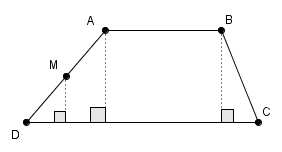
\includegraphics[scale=0.9]{de11.png}
\end{minipage}
\begin{minipage}{0.58\textwidth}
Ta có, $d(M,CD)=\frac 12 d(A,CD)=\frac 12 d(B,CD)$. \\
Nên $S_{\Delta BCD}=\frac 12.d(B,CD).BC=2d(M,CD).AB$. Từ đó tìm được $d(M,CD)=1$.\\
Khi đó ta sẽ viết được phương trình đường thẳng $CD$ (là đường thẳng qua $C$ cách $M$ một khoảng không đổi).
\end{minipage}

Cụ thể, gọi VTPT của $CD$ là $\vt{n}=(a,b)\neq \vt{0}$, phương trình của $CD$ là $a(x+1)+b(y+1)=0$, suy ra
$$ d(M,CD)=\frac{|2a-b|}{\sqrt{a^2+b^2}}=1\iff  3a^2-4ab=0\iff \hoac{a=0\\ 3a=4b}. $$
Với $a=0$, chọn $b=1$, ta được $CD$: $y+1=0$. Với giả thiết $CD=8$ và $x_D$ nguyên dương ta sẽ tìm được $D(7;-1)$. Mà $2\vt{AB}=\vt{DC}$ nên $B(-9;-3)$.\\
Với $3a=4b$, chọn $a=4$, $b=3$, ta được $CD$: $4x+3y+7=0$, tương tự như trên ta thấy trường hợp này không có điểm $D$ nào thỏa mãn điều kiện $x_D$ nguyên dương.

\deda{
Giải hệ phương trình $\hpt{2+9.3^{x^2-2y}=(2+9^{x^2-2y}).5^{2y-x^2+2}\quad (1)\\ 4^x+4=4x+4\sqrt{2y-2x+4}\quad (2)}.$
}
\hda 
Đk: $y-x+2\ge 0$. Với $(1)$ đặt $t=x^2-2y$ ta biến đổi thành
$$ \dfrac{2+3^{t+2}}{5^{t+2}}=\dfrac{2+3^{2t}}{5^{2t}}\iff  f(t+2)=f(2t). $$
Với $f(u)=\dfrac{2+3^u}{5^u}=2.\left(\dfrac 15\right)^u+\left(\dfrac 35\right)^u$ là hàm số nghịch biến trên $\mathbb R$ nên ta được $t=2\iff  2y=x^2-2$. Thế vào $(2)$ ta được
$$ 4^x+4=4x+4\sqrt{x^2-2x+2}\iff  4^{x-1}=x-1+\sqrt{(x-1)^2+1}\iff  4^s=s+\sqrt{s^2+1}.\quad (3) $$
Do $(s+\sqrt{s^2+1})(\sqrt{s^2+1}-1)=1$ nên $4^{-s}=\sqrt{s^2-1}-s$.\quad $(4)$.\\
Trừ vế $(3)$, $(4)$ ta được $4^{s}-4^{-s}-2s=0$.\quad $(\ast)$\\
Xét $g(v)=4^v-4^{-v}-2v$, $g'(v)=\ln 4(4^v+4^{-v})-2\ge 2\ln 4-2>0$. Suy ra $g(v)$ là hàm đồng biến, và do đó $(\ast)$ có đúng 1 nghiệm $s=0$. Và nghiệm hệ là $\left(1;-\frac 12\right)$.
% Nx: Bài toán hơi lắt léo.
\deda{
Cho $x,y,z>0$ thỏa mãn $x+y+1=z$. Tìm GTNN
$$ P=\dfrac{x}{x+yz}+\dfrac{y}{y+zx}+\dfrac{z^2+2}{z+xy}. $$
}
\hda 
Ta có $x+yz=yz-z-y-1=(z-1)(y+1)=(x+y)(y+1)$. Tương tự cũng có
$y+zx=(x+y)(x+1)$ và $z+xy=(x+1)(y+1)$. Nên
$$ P=\frac x{(x+y)(y+1)}+\frac{y}{(x+y)(x+1)}+\frac{z^2+2}{(x+1)(y+1)}=\frac{x^2+y^2+x+y}{(x+y)(x+1)(y+1)}+\frac{z^2+2}{(x+1)(y+1)}. $$
Lại có, $x^2+y^2\ge\frac 12(x+y)^2$; $(x+1)(y+1)\le \frac 14(x+y+2)^2$. Nên
$$ P\ge \frac{2(x+y)^2+4(x+y)}{(x+y+2)^2(x+y)}+\frac{4(z^2+2)}{(x+y+2)^2}=\frac{2(x+y)+4}{(x+y+2)^2}+\frac{4(z^2+2)}{(x+y+2)^2}=\frac{2}{z+1}+\frac{4(z^2+2)}{(z+1)^2}=f(z). $$
Xét $f(z)$ với $z>1$ ta sẽ suy ra được $f(z)\ge \frac{13}4$ hay $P_{\min}=\frac{13}4$ khi $x=y=1$, $z=3$.
\section{Đề 12}

\deda{
\bd cho tam giác $ABC$. Đường phân giác trong góc $A$ có phương tình $d$: $x-y+2=0$, đường cao hạ từ $B$ có phương trình $d'$: $4x+3y-1=0$. Biết hình chiếu của $C$ lên $AB$ là điểm $H(-1;-1)$. Tìm tọa độ $B,C$.
}
\hda 
\begin{minipage}{0.4\textwidth}
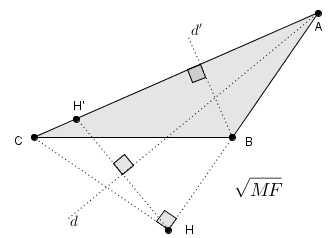
\includegraphics[scale=0.8]{de12.png}
\end{minipage}
\begin{minipage}{0.58\textwidth}
Một bài tập cơ bản minh họa cho phương pháp dựng hình. Các yếu tố cho trước: $d$, $d'$, $H$.\\
Từ đó, ta sẽ "dựng" được $H'$ (tức là tìm được tọa độ) đối xứng với $H$ qua $d$. Do $d$ là đường phân giác trong $\goc{BAC}$ nên $H'\in AC$. Từ đó ta sẽ dựng được đường thẳng $AC$ qua $H'$ vuông góc với $d'$.\\
$A=AC\cap d$, ta dựng được đường thẳng $AH$, $B=AH\cap d'$. Ta cũng dựng được đường thẳng $CH$ qua $H$ vuông góc $AB$ và $C=CH\cap AC$.
\end{minipage}

Với phân tích như thế, ta sẽ tìm được $B\left(0;\frac 13\right)$, $C\left(-\frac{10}3;\frac 34\right)$.

\deda{
Giải hệ phương trình $\hpt{xy(x+1)=x^3+y^2+x-y\quad (1)\\ 3y(2+\sqrt{9x^2+3})+(4y+2)(\sqrt{1+x+x^2}+1)=0\quad (2)}$.
}
\hda 
Với $(1)$, phân tích thành nhân tử ta sẽ được $(x-y)(x^2-y+1)=0\iff  \hoac{y=x\\ y=x^2+1}$.\\
Với $y=x^2+1$ thế vào $(2)$ dễ thấy vô nghiệm.\\
Với $y=x$ thế vào $(2)$ ta được
$$ 3x(2+\sqrt{9x^2+3})+(4x+2)(\sqrt{1+x+x^2}+1)=0$$ 
$$\iff  3x(2+\sqrt{9x^2+3})=(-2x-1)(\sqrt{3+(-2x-1)^2}+2)\iff  f(3x)=f(-2x-1) $$
Với $f(t)=t(\sqrt{t^2+2})$ là một hàm đồng biến nên ta được $3x=-2x-1\iff  x=-\frac 15$.\\
Nghiệm hệ là $\left(-\frac 15;-\frac 15\right)$.
\deda{
Cho $a,b,c>0$ thỏa mãn $a+b+c=2$. Tìm GTLN
$$ S=\sqrt{\dfrac{ab}{ab+2c}}+\sqrt{\dfrac{bc}{bc+2a}}+\sqrt{\dfrac{ca}{ca+2b}}. $$
}
\hda 
Ta có
$$ \sqrt{\frac{ab}{ab+2c}}=\sqrt{\frac{ab}{ab+(a+b+c)c}}=\sqrt{\frac{ab}{(a+c)(b+c)}}\le \frac 12\left(\frac{a}{a+c}+\frac{b}{b+c}\right). $$
Đẳng thức xảy ra khi $\frac{a}{a+c}=\frac{b}{b+c}$. Tương tự ta cũng có 
$$ \sqrt{\frac{bc}{bc+2a}}\le\frac 12\left(\frac b{b+a}+\frac c{c+a}\right);\quad \sqrt{\frac{ca}{ca+2b}}\le\frac 12\left(\frac c{c+b}+\frac{a}{a+b}\right). $$
Cộng các vế ta được $$S\le \frac 12\left(\frac{a+b}{a+b}+\frac{b+c}{b+c}+\frac{c+a}{c+a}\right)=\frac 32.$$
Vậy $S_{\max}=\frac 32$ khi $a=b=c=\frac 23$.
\section{Đề 13}

\deda{
Giải hệ phương trình $\hpt{y^2-x\sqrt{\dfrac{y^2+2}{x}}=2x-2\quad (1)\\ \sqrt{y^2+1}+\sqrt[3]{2x-1}=1\quad (2)}$.
}
\hda 
Đk: $x>0$. Với $(1)$, chia cả hai vế cho $x$ ta được
$$ \dfrac{y^2+2}{x}-\sqrt{\dfrac{y^2+2}x}-2=0\iff  \sqrt{\dfrac{y^2+2}{x}}=2\iff  y^2=4x+2. $$
Thế vào $(2)$ được $\sqrt{4x-1}+\sqrt[3]{2x-1}=1$.\\
Đặt $\sqrt{4x-1}=u\ge 0$; $\sqrt[3]{2x-1}=v$. Ta được $\hpt{u+v=1\\ u^2-2v^3=1}\iff  \hpt{u=1\\ v=0}$.\\
Từ đó ta được nghiệm hệ $\left(\frac 12;0\right)$.
\deda{
 \bd cho $A(2;1)$, $B(-1;-3)$ và hai đường thẳng $d_1$: $x+y+3=0$, $d_2$: $x-5y-16=0$. Tìm tọa độ $C\in d_1$ và $D\in d_2$ sao cho $ABCD$ là hình bình hành.
}
\hda 
Ta có, $C(c;-c-3)\in d_1$, $D(5d+16;d)\in d_2$ nên $\vt{CD}=(5d+16-c;d+c+3)$.\\
Do $ABCD$ là hình bình hành nên $\vt{BA}=\vt{CD}$ từ đó ta tìm được $d=-2$, $c=3$ và $C(3;-6)$, $D(6;-2)$.

\deda{
Cho $x,y\in \mathbb{R}$ thỏa mãn $x^2+y^2+xy=3$. Tìm GTLN và GTNN $P=x^3+y^3-3x-3y$.
}
\hda 
Ta có
$$ P=x^3+y^3-3x-3y=(x+y)^3-3xy(x+y)-3(x+y). $$
Lại có $x^2+y^2+xy=3\iff  xy=(x+y)^2-3$, nên
$$ P=t^3-3(t^2-3)t-3t=-2t^3+6t=f(t). $$
Với $t=x+y$. Mà $t^2-3=xy\le\frac{(x+y)^2}{4}=\frac{t^2}4$, nên $t\in[-2;2]$.\\
Xét $f(t)$ với $t\in[-2;2]$ ta tìm được $P_{\max}=4$, $P_{\min}=-4$.
\section{Đề 14}

\deda{
\bd cho hình vuông $ABCD$. $F\left(\dfrac{11}2;3\right)$ là trung điểm $AD$. $EK$: $19x-8y-18=0$ với $E$ là trung điểm $AB$, $K$ thuộc cạnh $CD$ sap cho $KD=3KC$. Tìm tọa độ $C$ biết $x_E<3$.
}
\hda
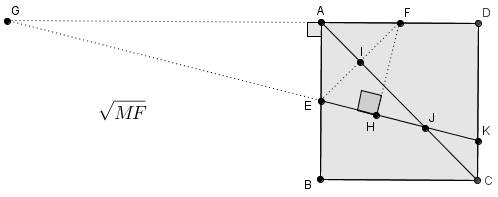
\includegraphics[scale=0.8]{de14.png}\\
Kẻ $FH\bot EK$, $FH=d(F, EK)=\frac{25}{2\sqrt{17}}$.\\
Gọi $G=AD\cap EK$, hình vuông có độ dài cạnh là $a$. Ta tính được $GE=\frac{a\sqrt{17}}2$, $GF=\frac{5a}2$. Hơn nữa, $\frac{AE}{FH}=\frac{GE}{GF}=\frac{\sqrt{17}}5$. Nên ta sẽ tính được $a=5$.\\
Khi đó $EF=\frac{5\sqrt 2}2$, mà $E\in EF$, $x_E<3$ nên ta tìm được $E\left(2;\frac 52\right)$.\\
Gọi $I\left(\frac{15}4;\frac{11}4\right)$ là trung điểm $EF$, suy ra $AC$: $7x+y-29=0$ (qua $I$ vuông góc với $EF$).\\
Gọi $P=AC\cap EF$, ta tìm được $P\left(\frac{10}3;\frac{17}3\right)$, hơn nữa $\vt{IC}=\frac 95\vt{IP}$ nên $C(3;8)$.



\deda{
Giải hệ phương trình $\hpt{|x-2y|+1=\sqrt{x-3y}\\ x(x-4y+1)+y(4y-3)=5}$.
}
\hda 
Đk: $x\ge 3y$. Đặt $|x-2y|=u\ge 0$; $|\sqrt{x-3y}|=v\ge 0$. ta được hệ
$$ \hpt{u-v=-1\\ u^2+v^2=5}\iff  \hpt{u=1\\v=2}. $$
Từ đó giải hệ ta được nghiệm $(-5;-3)$; $(-11;-5)$.
\deda{
Cho $a,b,c>0$. CMR
$$ \dfrac{a^2+1}{4b^2}+\dfrac{b^2+1}{4c^2}+\dfrac{c^2+1}{4a^2}\ge \dfrac{1}{a+b}+\dfrac{1}{b+c}+\dfrac{1}{c+a}. $$
}
\hda 
Ta có
\begin{eqnarray*}
VT&=&\left(\frac{a^2}{4b^2}+\frac 1{4b^2}\right)+\left(\frac{b^2}{4c^2}+\frac{1}{4c^2}\right)+\left(\frac{c^2}{4a^2}+\frac{1}{4a^2}\right)\\ 
&=&\frac{a}{2b^2}+\frac{b}{2c^2}+\frac{c}{2a^2}=\frac 12\left(\frac a{b^2}+\frac b{c^2}+\frac{c}{a^2}\right). 
\end{eqnarray*}
Mà
$$ \frac{a}{b^2}+\frac 1a\ge\frac 2b;\quad \frac{b}{c^2}+\frac 1b\ge \frac 2c;\quad \frac{c}{a^2}+\frac 1c\ge \frac 2a. $$
Nên
$$ \frac{a}{b^2}+\frac{b}{c^2}+\frac{c}{a^2}\ge \frac 1a+\frac 1b+\frac 1c. $$
Suy ra
$$ VT\ge \frac 12\left(\frac 1a+\frac 1b+\frac 1c\right)=\frac 14\left[\left(\frac 1a+\frac 1b\right)+\left(\frac 1b+\frac 1c\right)+\left(\frac 1c+\frac 1a\right)\right]\ge \frac 14\left( \frac 4{a+b}+\frac 4{b+c}+\frac 4{c+a}\right)=VP. $$
Đẳng thức xảy ra khi $a=b=c=1$.
\section{Đề 15}

\deda{
\bd cho hình thang $ABCD$ vuông tại $A,D$; diện tích hình thang bằng $6$; $CD=2AB$, $B(0;4)$. Biết $I(3;-1)$, $K(2;2)$ lần lượt nằm trên đường thẳng $AD$ và $DC$. Viết phương trình đường thẳng $AD$ biết $AD$ không song song với trục tọa độ.
}
\hda 
Vì $AD$ không song song với các trục tọa độ nên gọi VTPT của $AD$ là $\vt{n}=(1,a)$ $(a\neq 0)$.\\
Suy ra $AD$: $x+ay+a-3=0$ và $DC$: $ax-y-2a+2=0$.\\
Từ đó ta tính được $d(B,DC)=\frac{|2a+2|}{\sqrt{a^2+1}}$, $d(B,AD)=\frac{|5a-3|}{\sqrt{a^2+1}}$.\\
Mà $S_{ABCD}=\frac 12AD.(AB+CD)=6$ nên ta sẽ tìm được $a=1$, $a=-\frac 53$, $a=\frac{-1\pm2\sqrt 2}7$.

\deda{
Giải hệ phương trình $\hpt{x+\sqrt{x(x^2-3x+3)}=\sqrt[3]{y+2}+\sqrt{y+3}+1\quad (1)\\ 3\sqrt{x-1}-\sqrt{x^2-6x+6}=\sqrt[3]{y+2}+1\quad (2)}$.
}
\hda 
Đk: $x\in [1;3-\sqrt{3}]\cup [3+\sqrt 3;+\infty)$; $y\in[-3;+\infty)$.\\
$$ (1)\iff  x-1+\sqrt{(x-1)^3+1}=\sqrt[3]{y+2}+\sqrt{(\sqrt[3]{y+2})^3+1}\iff  f(x-1)=f(\sqrt[3]{y+2}). $$
Với $f(t)=t+\sqrt{t^3+1}$, $t\ge -1$  là hàm đồng biến nên ta có $x-1=\sqrt[3]{y+2}$. Thế vào $(2)$ ta được
$$ 3\sqrt{x-1}-\sqrt{x^2-6x+6}=(x-1)+1\iff  (x-1)+1+\sqrt{(x-1)^2-4(x-1)+1}=3\sqrt{x-1}. $$
Do $x=1$ không thỏa mãn nên chia cả hai vế cho $\sqrt{x-1}>0$ ta được
$$ \sqrt{x-1}+\dfrac{1}{\sqrt{x-1}}+\sqrt{x-1-4+\dfrac 1{x-1}}=3\iff  t+\sqrt{t^2-6}=3\iff  t=\dfrac 52. $$
Với $t=\sqrt{x-1}+\dfrac{1}{x-1}>2$. Từ đó ta tìm được nghiệm hệ $(5;62)$, $\left(\frac 54;-\frac{127}{64}\right)$.
\deda{
Cho $x,y>0$ thỏa mãn $x-y+1\le 0$. Tìm GTLN
$$ T=\dfrac{x+3y^2}{\sqrt{x^2+y^4}}-\dfrac{2x+y^2}{5x+5y^2}. $$
}
\hda 
Ta có $x\le y-1\implies  0<\frac x{y^2}\le\frac 1y-\frac 1{y^2}=\frac 14-\left(\frac 1y-\frac 12\right)^2\le \frac 14$. Đặt $t=\frac{x}{y^2}\implies  t\in(0;\frac 14]$.\\
Suy ra
$$ T=\frac{\frac{x}{y^2}+3}{\sqrt{\left(\frac{x}{y^2}\right)^2+1}}-\frac 15\cdot\frac{2\frac{x}{y^2}+1}{\frac{x}{y^2}+1}=\frac{t+3}{\sqrt{t^2+1}}-\frac 15\cdot\frac{2t+1}{t+1}=f(t). $$
$$ f'(t)=\frac{1-3t}{\sqrt{(t^2+1)^3}}-\frac 15\cdot\frac{1}{(t+1)^2}. $$
Do $t\in(0;\frac 14]$ nên $1-3t\ge \frac 14$; $\sqrt{(t^2+1)^3}\le \sqrt{\left(\frac{17}{16}\right)^3}\implies  \frac{1-3t}{\sqrt{(t^2+1)^3}}\ge \frac{4}{17\sqrt{\frac{17}{16}}}$.\\
Và $-\frac 15\cdot\frac{1}{(t+1)^2}>-\frac 15$. Suy ra $f'(t)>0$.\\
Vậy $f(t)$ đồng biến trên $(0;\frac 14]\implies  f(t)\le f(\frac 14)=\frac{13}{\sqrt{17}}-\frac 6{25}$.